\subsection{电商环境}
\label{subsec:ecommerce}
除了竞争性博弈之外，电商中的顾客—智能体交互也是一个非常贴近现实的场景，在这里推测动作能够显著改善性能。典型工作流中，顾客通过聊天界面提交请求，然后等待智能体响应。当智能体需要顺序调用多个 API 时——例如处理退货可能需要先获取订单信息、再验证每件商品的退货资格、最后发起退货——由此产生的延迟会明显损害用户体验。相反，如果某些 API 调用能够被正确推测并提前执行，那么在用户请求真正到达时，智能体就可以立即返回结果，从而大幅降低延迟，使交互体验更加顺滑。我们在 \emph{$\tau$-bench} 的零售环境上评估这一设置\cite{yao_Taubench_2024}。

\subsubsection{实验设置}
\paragraph{推测流水线}
在该场景下，当前状态 $s_t$ 定义为截至回合 $t$ 的对话历史，而 $h_t$ 表示为回答用户查询所需调用的 API（例如 \texttt{get\_user\_details}、\texttt{get\_order\_details}）。我们的 Speculator 将预测：
\begin{enumerate}
    \item 用户的查询 $\hat{a}_t$；
    \item 在当前状态 $s_t$ 与第 1 步得到的用户查询预测共同条件下，对应的目标 API 调用及其参数 $(\hat{h}_{t+1}^{(i)}, \hat{q}_{t+1}^{(i)})$，其中 $i \in \{1, \ldots, k\}$。由于每个回合需要的 API 调用数并不固定，Speculator 还必须同时预测 $k$。
\end{enumerate}

\paragraph{智能体配置}
我们测试了多种 Speculator 模型：OpenAI GPT 系列（gpt-5-nano、gpt-5-mini、gpt-5）以及 Google Gemini 系列（gemini-2.5-flash），并设置不同的推理预算（1024、2048、4096 tokens）。
已有工作\cite{jiang-etal-2023-llm, chen_LLMEnsemble_2025} 表明，异构 LLM 集成通常优于单一模型，而且多个模型可以在相同时间预算下并行执行。受此启发，我们评估了两种 Speculator 配置：(i) \emph{单模型}设置，即推测仅依赖一个模型；(ii) \emph{多模型}设置，即让能力与推理预算相近的模型并行运行（例如 gpt-5-nano 搭配低预算 Gemini，gpt-5-mini 搭配中预算 Gemini，以及 gpt-5 搭配高预算 Gemini）。随后，它们的预测会被汇总为一个共享的推测动作候选集合。在运行时，当用户模拟器给出真实输入后，Actor 会将推测得到的 API 调用与真实所需 API 进行比较。正确的预测会被立即提交，从而消除延迟；错误的预测则被安全丢弃，不影响正确性。

\paragraph{评估}
我们使用\textbf{API 预测准确率}来衡量性能，即推测出的 API 调用中，有多少比例与解决用户问题所需的真实 API 调用相匹配。该指标直接反映了用户在多少比例的回合中能够立刻得到响应，而无需等待 API 真正执行。换言之，更高的预测准确率会直接转化为更大的时间收益。

\subsubsection{结果}

\begin{wrapfigure}{r}{0.45\columnwidth}
\vspace{-3ex}
    \centering
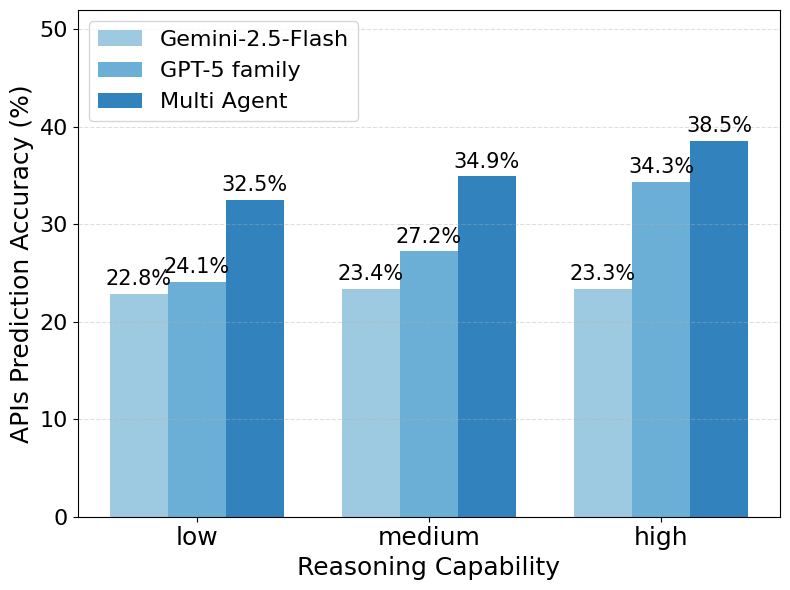
\includegraphics[width=\linewidth]{figures/ecommerce/pred_acc2.png}
    \caption{不同 Speculator 模型在不同推理能力设置下的 API 预测准确率。}
    \label{fig:pred_acc}
    \vspace{-30pt}
\end{wrapfigure}

\cref{fig:pred_acc} 表明，Speculator 能够正确预测 22\% 到 38\% 的 API 调用。随着模型能力增强，准确率会提升；同时，多模型配置也稳定优于单模型推测。更重要的是，低预算模型完成一次推测只需 2--3 秒（依据 LLM API providers leaderboard\footnote{\url{https://artificialanalysis.ai/leaderboards/providers}}），远低于平均约 30 秒的用户打字时间（按每分钟 40 个词估算）。这意味着，在约三分之一的回合中，智能体都可以比顺序执行更快地响应，而无需等待 API 执行完成。上述结果说明，在工具密集型环境中，推测可以把原本明显滞后的用户体验，转变为接近实时的交互。
